
\chapter{Analysis of results}
\label{chap:analysis}


\section{Results}

In the system represented before, I represent the cyber defense. On the same system, Justin Bouroux achieved
attacks and tried to penetrate the system. Of course, it was designed to have some security issues, but the most
important for my system is the detection of its attacks. In fact, all system have security issue even the most
secure\footnote{A minimum of <<zero day>>}, but if we can detect an intrusion we are able to ensure the service. If
you want more information about attacks carried out, you can read the Justin's report.
~\\

To begin, when an hacker want to attack a system he always tries to scan the ports. We can notice that my system
was able to detect the scan of ports. You can see on the next figure that Suricata raised some warnings during the
scan. This warnings represent a possible attacks. It is very important to detect that because it is often the
synonym that someone want to attack your system.

\begin{figure}[h]
  \centering
  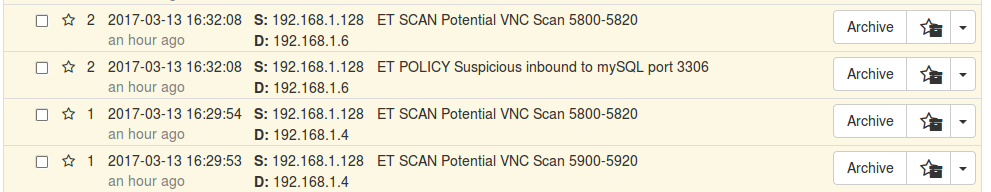
\includegraphics[width=\textwidth]{scan}
  \caption{Events raised during the scan}
  \label{fig:scan}
\end{figure}



Then, he has tested the application <<ping-pong>>. On the next figure, it is possible to see the messages
<<go\_ping>> and <<go\_pong>> catch by the IDS. The events are raised because I had the rules described on the
section \ref{sec:rules}.

\begin{figure}[h]
  \centering
  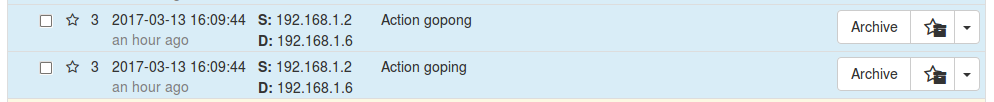
\includegraphics[width=\textwidth]{goping_gopong}
  \caption{Events goping and gopong}
  \label{fig:gopong}
\end{figure}


Justin, also try to access to the admin interface with the combination of <<to\_ping>>, <<to\_pong>>, and
<<admin>>. It is possible to notice, that my system of detection is able to detect this attack. On the network the
attack seems invisible because he isn't logged in the port 9000, but the application send the event <<appli-python:
go to admin state>>. So, my SIEM understand that the user has access to the admin interface without using the good
interface, so there is a problem: our system is under attack.

\begin{figure}[h]
  \centering
  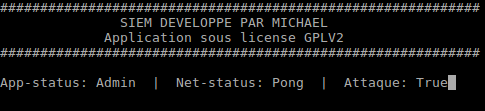
\includegraphics[width=0.7\textwidth]{admin_fuz}
  \caption{SIEM interface}
  \label{fig:fuzz}
\end{figure}


And to finish, Justin hacked the metasploitable computer to have access to the admin interface on the port 9000.
After his attack, my system of detection raise a lot of alert. Firstly, because the IDS has detected his attack
against the metasploitable. Secondly, because the application has raised event when he arrived on the admin
interface. So, I am able to identify his attack against the metasploitable and connect it to the access of the
admin interface.


\begin{figure}[h]
  \centering
  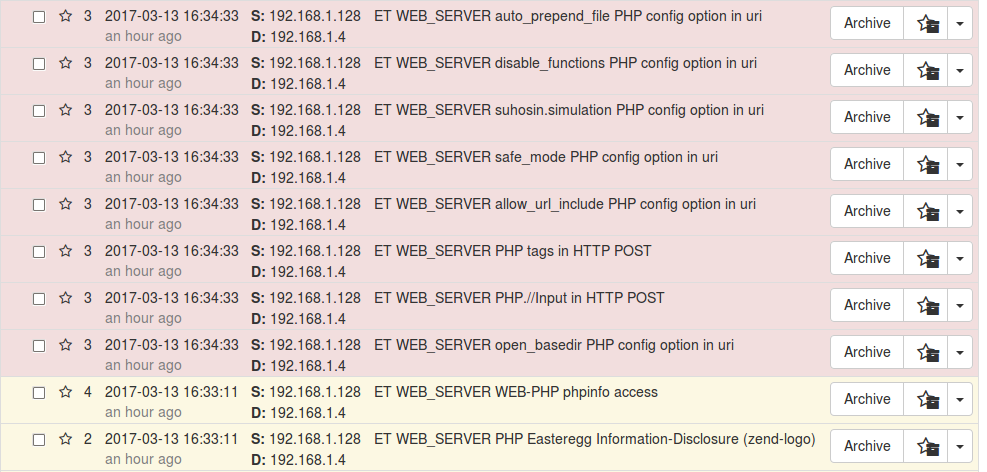
\includegraphics[width=\textwidth]{attacks}
  \caption{Alerts during metasploitable attacks}
  \label{fig:attcks}
\end{figure}

A demonstration video will be presented during the presentation.


\section{Way of improve}

To summarize, during this test phase I was able to detect all attacks. However, I had some issue. In fact, the
Suricata IDS sometimes raises event later. Sometimes 5 minutes after the real event. It is not a problem for a
normal IDS, but for our utilization it is. We want to know the states of our system without delay to analyze them.
Even if I think the problem can be solved with computer more efficient, it is a real issue.

Moreover, I didn't protect my detector system because of the lack of time, so it is possible to attack it. For
example, it is possible to send false messages to the SIEM to hide attacks. It would be necessary to add an
authenticity on the messages send by the application to the SIEM.

Finally, we can notice that my system is very huge and very complex. So the transition to scale could be very hard.
So the system need some improvements in this direction as well.



%%% Local Variables:
%%% mode: latex
%%% TeX-master: "../rapport_de_base"
%%% End:
